
%% bare_jrnl_compsoc.tex
%% V1.4b
%% 2015/08/26
%% by Michael Shell
%% See:
%% http://www.michaelshell.org/
%% for current contact information.
%%
%% This is a skeleton file demonstrating the use of IEEEtran.cls
%% (requires IEEEtran.cls version 1.8b or later) with an IEEE
%% Computer Society journal paper.
%%
%% Support sites:
%% http://www.michaelshell.org/tex/ieeetran/
%% http://www.ctan.org/pkg/ieeetran
%% and
%% http://www.ieee.org/

%%*************************************************************************
%% Legal Notice:
%% This code is offered as-is without any warranty either expressed or
%% implied; without even the implied warranty of MERCHANTABILITY or
%% FITNESS FOR A PARTICULAR PURPOSE! 
%% User assumes all risk.
%% In no event shall the IEEE or any contributor to this code be liable for
%% any damages or losses, including, but not limited to, incidental,
%% consequential, or any other damages, resulting from the use or misuse
%% of any information contained here.
%%
%% All comments are the opinions of their respective authors and are not
%% necessarily endorsed by the IEEE.
%%
%% This work is distributed under the LaTeX Project Public License (LPPL)
%% ( http://www.latex-project.org/ ) version 1.3, and may be freely used,
%% distributed and modified. A copy of the LPPL, version 1.3, is included
%% in the base LaTeX documentation of all distributions of LaTeX released
%% 2003/12/01 or later.
%% Retain all contribution notices and credits.
%% ** Modified files should be clearly indicated as such, including  **
%% ** renaming them and changing author support contact information. **
%%*************************************************************************


% *** Authors should verify (and, if needed, correct) their LaTeX system  ***
% *** with the testflow diagnostic prior to trusting their LaTeX platform ***
% *** with production work. The IEEE's font choices and paper sizes can   ***
% *** trigger bugs that do not appear when using other class files.       ***                          ***
% The testflow support page is at:
% http://www.michaelshell.org/tex/testflow/


\documentclass[10pt,journal,compsoc]{IEEEtran}
%
% If IEEEtran.cls has not been installed into the LaTeX system files,
% manually specify the path to it like:
% \documentclass[10pt,journal,compsoc]{../sty/IEEEtran}





% Some very useful LaTeX packages include:
% (uncomment the ones you want to load)


% *** MISC UTILITY PACKAGES ***
%
%\usepackage{ifpdf}
% Heiko Oberdiek's ifpdf.sty is very useful if you need conditional
% compilation based on whether the output is pdf or dvi.
% usage:
% \ifpdf
%   % pdf code
% \else
%   % dvi code
% \fi
% The latest version of ifpdf.sty can be obtained from:
% http://www.ctan.org/pkg/ifpdf
% Also, note that IEEEtran.cls V1.7 and later provides a builtin
% \ifCLASSINFOpdf conditional that works the same way.
% When switching from latex to pdflatex and vice-versa, the compiler may
% have to be run twice to clear warning/error messages.






% *** CITATION PACKAGES ***
%
\ifCLASSOPTIONcompsoc
  % IEEE Computer Society needs nocompress option
  % requires cite.sty v4.0 or later (November 2003)
  \usepackage[nocompress]{cite}
\else
  % normal IEEE
  \usepackage{cite}
\fi





% *** GRAPHICS RELATED PACKAGES ***
%
\ifCLASSINFOpdf
  \usepackage[pdftex]{graphicx}
  % declare the path(s) where your graphic files are
  \graphicspath{{./assets/}}
  % and their extensions so you won't have to specify these with
  % every instance of \includegraphics
  \DeclareGraphicsExtensions{.pdf,.jpeg,.png}
\else
  % or other class option (dvipsone, dvipdf, if not using dvips). graphicx
  % will default to the driver specified in the system graphics.cfg if no
  % driver is specified.
  % \usepackage[dvips]{graphicx}
  % declare the path(s) where your graphic files are
  % \graphicspath{{../eps/}}
  % and their extensions so you won't have to specify these with
  % every instance of \includegraphics
  % \DeclareGraphicsExtensions{.eps}
\fi
% graphicx was written by David Carlisle and Sebastian Rahtz. It is
% required if you want graphics, photos, etc. graphicx.sty is already
% installed on most LaTeX systems. The latest version and documentation
% can be obtained at: 
% http://www.ctan.org/pkg/graphicx
% Another good source of documentation is "Using Imported Graphics in
% LaTeX2e" by Keith Reckdahl which can be found at:
% http://www.ctan.org/pkg/epslatex
%
% latex, and pdflatex in dvi mode, support graphics in encapsulated
% postscript (.eps) format. pdflatex in pdf mode supports graphics
% in .pdf, .jpeg, .png and .mps (metapost) formats. Users should ensure
% that all non-photo figures use a vector format (.eps, .pdf, .mps) and
% not a bitmapped formats (.jpeg, .png). The IEEE frowns on bitmapped formats
% which can result in "jaggedy"/blurry rendering of lines and letters as
% well as large increases in file sizes.
%
% You can find documentation about the pdfTeX application at:
% http://www.tug.org/applications/pdftex




\hyphenation{op-tical net-works semi-conduc-tor}


\begin{document}
%
% paper title
% Titles are generally capitalized except for words such as a, an, and, as,
% at, but, by, for, in, nor, of, on, or, the, to and up, which are usually
% not capitalized unless they are the first or last word of the title.
% Linebreaks \\ can be used within to get better formatting as desired.
% Do not put math or special symbols in the title.
\title{SD-NFV as an Energy Efficient Approach \\
       for M2M Networks Using \\
       Cloud-Based 6LoWPAN Testbed}

\author{Michel Massamiri,
        Kenji Fontaine}% <-this % stops a space}

\IEEEtitleabstractindextext{%
% Note that keywords are not normally used for peerreview papers.
\begin{IEEEkeywords}
M2M, IoT, NFV, SDN, SD-NFV, energy efficiency, 6LoWPAN \\
\end{IEEEkeywords}}


% make the title area
\maketitle


\IEEEdisplaynontitleabstractindextext
\IEEEpeerreviewmaketitle



\section{Introduction}\label{sec:introduction}

In this ever growing interconnected world, Machine-to-Machine (M2M) 
communication is a key technology to build the Internet-of-Things (IoT). 
M2M nodes are characterized by their limited power, making energy 
efficiency one of the most important factor for the growth of this 
technology. 

The IoT can be divided into 4 different layers. The first layer is called 
the \textit{sensing layer}. This layer is mainly composed of 
sensors that will collect informations about temperature, humidity, 
chemicals in the air, pressure, etc. that will be 
collected by the second layer. The second layer is called the 
\textit{aggregation layer}. The third layer is the processing layer. Its 
purpose is to apply further processing to the data that have been sent by 
the aggregation layer. After the processing is completed, the data can 
be uploaded to the fourth layer, \textit{the cloud layer}. This will 
allow the data to be used for various applications.

IoT applications are based on a large number of M2M nodes. 
Having this many M2M nodes leads to difficulty in 
managing and controling the network. Software defined networking (SDN) 
and Network functioning visualisation (NFV) are potential solutions to 
these problems. Both SDN and NFV aim to make the network management 
of M2M nodes simpler and more flexible by adding programmability features. 
SDN enables sensor node to be retasked by splitting the control plane from 
the data plane. NFV focuses on reducing operating and capital expenses, 
by decoupling the network functions from the physical devices. 

This document focuses on analyzing the solution implemented by Bilal 
R. Al-Kaseem and Hamed S. Al-Raweshidy. This document will detail 
how SDN, NFV and cloud computing can be used together to improve the 
network management of a large amount of M2M nodes. 
The proposed approach is called customized software defined-NFV (SD-NFV). 
The experimental results have showed that the SD-NFV could reduce 
network discovery time by 60\% and extend M2M nodes' lifetime by 65\%.

\section{Context and Related Work}\label{sec:context}

This section introduces a few studies related to the integration and 
implementation of SDN and NFV in low-power networks using cloud 
computing services. Whilst there are a good number of studies dealing with 
either SDN or NFV, studies implementing an approach using both are 
rather scarce.

\textbf{Insert ref}

\section{Contribution}\label{sec:contribution}

As previously stated, studies using both SDN and NFV being rare, this paper 
focuses on validating the proof-of-concept of how SDN, NFV and cloud 
computing can be used to achieve greater efficiency in M2M-based networks.
The main contributions can be summarized as follows.

\begin{itemize}
    \item Designing a cost-effective M2M sensor node using 6LoWPAN 
    protocol alongside open source hardware and software;
    \item Building a custom SDN controller meetings the criterias of
    6LoWPAN regarding packet size and node discovery (ND);
    \item Delegating the adaptation layer from nodes to the centralized 
    SDN controller, effectively working as an edge router (or gateway) for 
    the cloud-based network;
    \item Providing global connectivity and data storage to the M2M sensor 
    network using a cloud-based platform through the M2M gateway.
\end{itemize}
The proposed approach is called customized SD-NFV. It provides a dynamic 
and scalable deployment for an M2M-based IoT application. The goal is 
to simplify network management by providing programmability features 
to the M2M network. The implemented testbed shows a significant 
improvement in reducing the energy consumption of M2M sensor nodes 
compared to the traditional approach.

\section{Discussion}\label{sec:discussion}
\subsection{to do}

This section details the implementation steps of the proposed SD-NFV 
architecture based on an 6LoWPAN testbed. The goal is to propose 
an energy-efficient way to improve the network lifetime by adding 
programmability feature. Hardware and software components choices 
will be detailed. The developed testbed has been integrated with a cloud 
computing platform to provide global access to the M2M sensor network.

\subsubsection{6LoWPAN hardware platform}

Each M2M sensor node is constitued of various subsystems, such as 
sensing, computation, communication and power. 6LoWPAN is an 
energy-efficient way to provide, small devices with limited energy, 
IPv6 connectivity. Over the last few years, there have been several 
propositions for 6LoWPAN. Most of them were using an operating system, 
where the 6LoWPAN protocol was being used on top of the operating system. 
However, M2M sensor are held back by their limited energy source and 
moderate memory size and processing power. Which makes running an OS 
on sensor nodes, not the most appropriate approach.

To meet the IoT promises, it is important for sensor nodes to be 
cost-effective and energy-efficient. There are several choices available, 
commercial or open source. The \textit{Arduino} has been the choice 
for this testbed, which is an open source microcontroller board. 
To comply with the IoT paradigm, it is mandatory for each nodes to be 
addressable, controlable and accessible via the Internet. M2M nodes 
communicate by using the IEEE 802.15.4 standard. In this 
experiment, Bilal R. Al-Kaseem and Hamed S. Al-Raweshidy opted for 
a simple temperature and humidity sensor that will forward these 
informations to the M2M gateway. The following figure shows M2M sensor 
nodes prototypes. Sensor nodes can be classified as follows.
\begin{itemize}
    \item \textbf{Simple Node :} Performs sensing and communication only. 
    They do not possess any processing capabilites and cannot be 
    selected as a cluster head. This type of nodes are composed of a 
    temperature sensor and powered by a 3.7 V/1000 mAh battery. 
    \item \textbf{Advanced Node :} Performs sensing, communication and 
    processing of the data collected by the sensors. They can be 
    definied as cluster head. This type of nodes are composed of a 
    temperature and humidity sensor attached to an Arduino Uno board. 
    They are powered by a 9 V/1600 mAh battery.
    \item \textbf{Sink Node :} This is the final destination for all the 
    data that has been been collected by the M2M sensor nodes. Depending 
    on the application, it can either be mobile or static. In this 
    experiment, an Arduino Uno board has been used. Sink nodes can 
    communicate with simple or advanced nodes. They also have an 
    Internet access, bringing cloud-based data storage to the M2M 
    network. The sink node is powered by a permanent source.
\end{itemize}

\begin{figure*}
    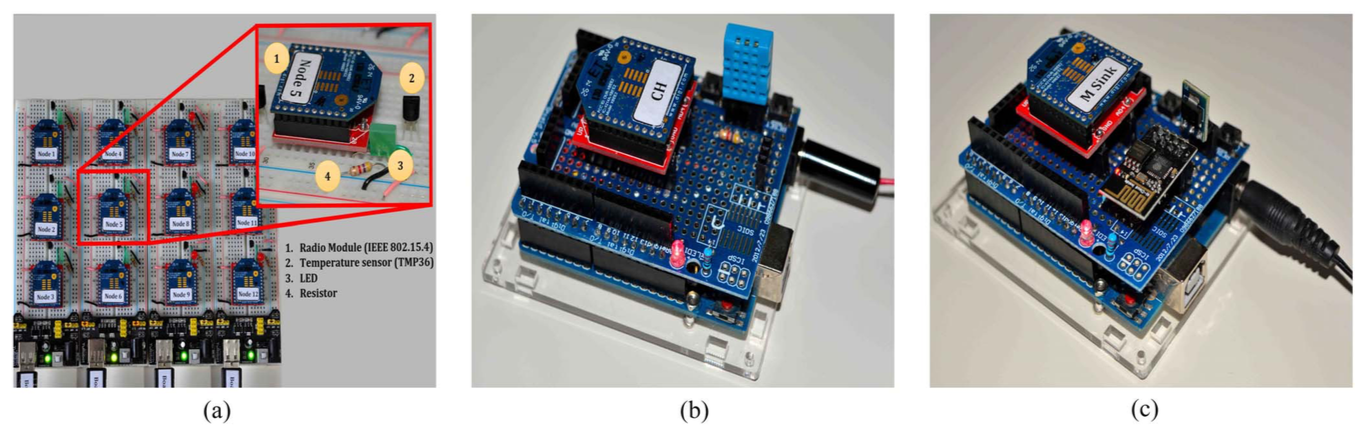
\includegraphics[width=\textwidth]{m2mnodes}
    \caption{M2M sensor nodes prototypes in the cloud-based 6LoWPAN 
    testbed. (a) Simple node (b) Advanced node (c) Sink node}
\end{figure*}

\subsubsection{Customized SDN Controller}

SDN and NFV share the same goal. They both endeavour to develop open 
software for standardized network hardware. The NFV technology aims to 
provide on-demande network functions and locate them on the most 
suitable location in the network. The SDN technology is used to split 
the control plane and data plane in order to increase the ability of 
the network to be programmable and reconfigurable. Whilst there are 
benefits using SDN or NFV individually, it is possible to use both to 
achieve further improvement. 

The proposed integration of SDN and NFV is aimed at deploying different 
routing algorithms for the 6LoWPAN network by using a VNF on top of 
the gateway. The SDN controller is a software-based network entity 
that allows the user to manage and control the network devices using 
an application programming interface (API). The customized SDN controller 
should consider the difference in processing capacity and the limited 
power of each node to achieve better efficiency. 

The SDN controller software is customized to fit a 6LoWPAN protocol stack, 
enabling end-to-end services on smaller devices. The controller is 
responsible for the following :

\begin{itemize}
    \item Discovering the network topology;
    \item Managing different services;
    \item Virtualization;
    \item Routing data and balancing loads.
\end{itemize}

The network discovery manager keeps the table entries up-to-date 
by periodically checking which nodes are available. It is important that 
the service manager takes into account each node's availability and 
capacity to assign services in efficient manner.

\subsubsection{Cloud computing services}

ThingSpeak is the cloud computing platform that was used in this 
experiment. It provides free storage alonside a data visualization 
feature. The cloud platform is connected to the 6LoWPAN network through 
the SD-NFV gateway. 

\subsubsection{Remote End-User Application}

In this experiment a simple MATLAB(MATLAB REF) application was used to 
emulate an external IP access to the 6LoWPAN network through the 
SD-NFV gateway. This application is used to receive the data from the 
cloud and to send control commands to the sensor nodes.

Figure 2 summarizes the general architecture of the proposed solution.

\begin{figure*}
    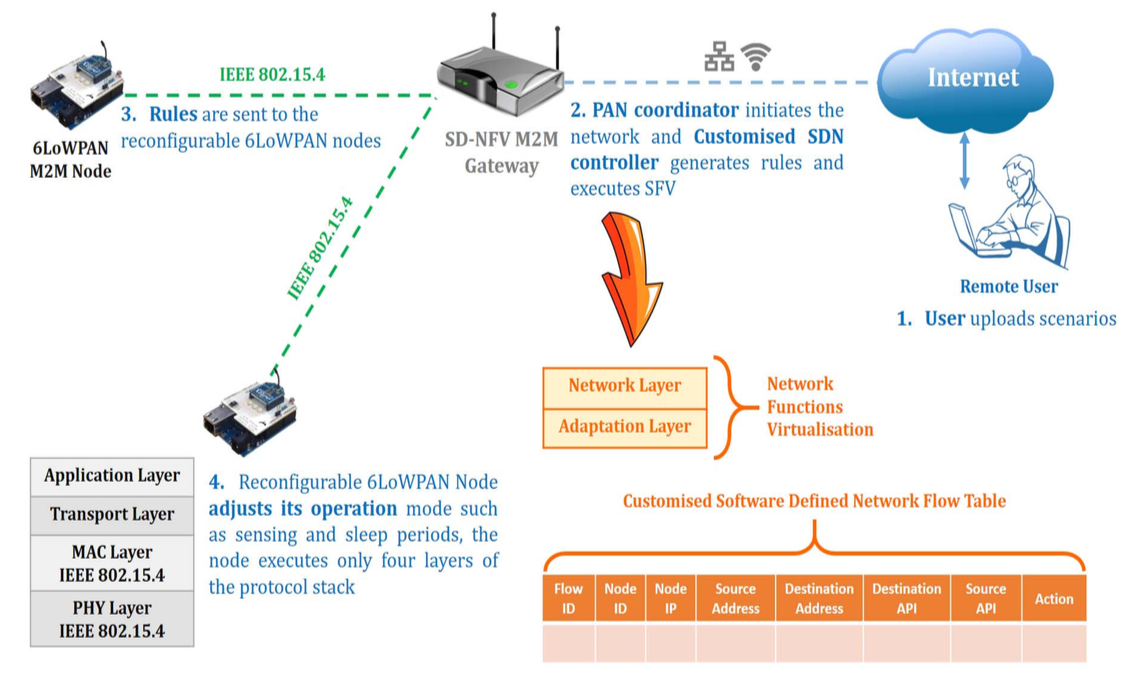
\includegraphics[width=\textwidth]{architecture}
    \caption{Architecture of the SD-NFV gateway using cloud-based 
    6LoWPAN testbed}
\end{figure*}

\subsection{Experimental results}

This section provides detailed proof-of-concept results for an 
implementation using SDN and NFV in a cloud-based M2M network. The 
tests were carried in indoor environments. 

\subsubsection{Node Discovery Phase}

It costs a lot of resources to manually discover each node in a 
6LoWPAN network. Having the SDN controller automatically monitor the 
states of all the nodes in the network constitutes a great improvement 
regarding the discovery time and thus, the node's lifetime. The figure 4 
shows the network discovery delay given a certain number of nodes. 
A very clear improvement can be seen on the graph. SD-NFV roughly 
reduces the discovery delay by 60\%. 

\subsubsection{Sensing Application}

The node lifetime is the time span from deployment to the instant when 
the node is considered non-functional or failed. Due to the limited 
energy source attached to the nodes, it is crucial to be efficient 
in energy usage. The experimental results focuses on the advanced nodes 
because they play the important of being a cluster head. Figure 5 
shows the difference in node lifetime with and without SD-NFV. 
SD-NFV manages to increase the node lifetime by approximately 65\% 
by limiting unnecessary packets transmission. Virtualizing the network 
in the SD-NFV gateway enable nodes to perform low-energy sleep mode in 
order to limit energy consumption. Figure 6 shows the node activity 
in relation to the node energy. With SD-NFV, nodes spend most of their 
time in idle mode, significantly increasing their lifetime.

\section{Conclusion}\label{sec:conclusion}


\appendices
\section{Proof of the First Zonklar Equation}
Appendix one text goes here.

\begin{thebibliography}{1}
\bibitem{IEEEhowto:kopka}
H.~Kopka and P.~W. Daly, \emph{A Guide to \LaTeX}, 3rd~ed.\hskip 1em plus
  0.5em minus 0.4em\relax Harlow, England: Addison-Wesley, 1999.
\end{thebibliography}

\end{document}


